\subsection{Thermal properties}
\label{sec:t_properties}

Thermal properties we have to consider are heat capacity $\HeatCapacity$ and thermal conductivity $\lambda$.
In the following we introduce the properties for gases and liquids separately.

%.........................................................................
\subsubsection{Specific heat capacity - $\HeatCapacity$}

Specific heat capacity is defined by the equations.
%
\begin{eqnarray}
\HeatCapacity_V
=
\frac{\p e}{\p\Temperature}
\quad , \quad
\HeatCapacity_p
=
\frac{\p\Enthalpy}{\p\Temperature}
\equiv
c
\end{eqnarray}

Therefore, specific enthalpy can be calculated from following relation.
%
\begin{eqnarray}
\Enthalpy(\Temperature)
=
\int_{T_0}^{T}
\HeatCapacity_p
d\theta
\end{eqnarray}

Heat capacity $c\rho$ of the composite porous medium
contains contributions of all involved phases.

\begin{eqnarray}
c\rho
=
(1-n)c^s\rho^s
+
\sum_\Phase S^\Phase c^\Phase \rho^\Phase
\label{eqn:heat_capacity}
\end{eqnarray}

%.........................................................................
\subsubsection{Thermal conductivity - $\lambda$}

Concuctive heat flux is assumed to be governed by Fourier's law
%
\begin{eqnarray}
\Flux_T
=
- 
\HeatConductivity(\Saturation,\Porosity)
\nabla\Temperature
\end{eqnarray}
%
where $\HeatConductivity$ is the overall thermal conductivity of the porous medium. Overall thermal conductivity depends on porosity and saturation and is given by a geometric mean approximation.
%

Thermal conductivity $\lambda$ of the composite porous medium
contains contributions of all involved phases.

\begin{itemize}
	\item Geometric mean
\begin{eqnarray}
\HeatConductivity
=
(\HeatConductivity^s)^{(1-\Porosity)}
\prod_\Phase
(\HeatConductivity^\Phase)^{\Porosity\Saturation^\Phase}
\end{eqnarray}

	\item Arithmetric mean
\begin{eqnarray}
\HeatConductivity
=
(1-n)\HeatConductivity^s
+
\sum_\Phase S^\Phase \HeatConductivity^\Phase
\label{eqn:thermal_conductivity}
\end{eqnarray}

\end{itemize}

%.........................................................................
\subsubsection{Gases}

Beside the hydraulic characteristics such as air viscosity, the thermal gas and solid properties such as heat capacity and thermal conductivity are important for heat transport.
As an example, Fig. \ref{fig:thermal_properties} depicts the thermal properties of the gaseous phase.
Fig. \ref{fig:thermal_properties} (left) shows the temperature dependence of specific heat capacity of air at atmospheric pressure corresponding to equation (\ref{eqn:heat_capacity}) from \cite{ZografosEtAl:1987} compared with experimental data by \cite{VargaftikEtAl:1996}. Fig. \ref{fig:thermal_properties} (right) illustrates the temperature dependence of thermal conductivity of air at atmospheric pressure corresponding to equation (\ref{eqn:thermal_conductivity}) from \cite{ZografosEtAl:1987} compared with experimental data by \cite{VargaftikEtAl:1996}. The pressure dependency of thermal properties can be neglected in the present pressure regimes.

\begin{eqnarray}
c^g
=
1.0613
&-&
4.3282 \times 10^{-4} T
\nonumber\\
&+&
1.0234 \times 10^{-6} T^2
\nonumber\\
&-&
6.4747 \times 10^{-10} T^3
\nonumber\\
&+&
1.3864 \times 10^{-13} T^4
\label{eqn:heat_capacity}
\end{eqnarray}

\begin{eqnarray}
\lambda^g
=
7.488 \times 10^{-3}
&-&
1.7082 \times 10^{-4} T
\nonumber\\
&+&
2.3758 \times 10^{-7} T^2
\nonumber\\
&-&
2.2012 \times 10^{-10} T^3
\nonumber\\
&+&
9.46 \times 10^{-14} T^4
\nonumber\\
&-&
1.579 \times 10^{-17} T^5
\label{eqn:thermal_conductivity}
\end{eqnarray}

\begin{figure}[htb!]
\begin{center}
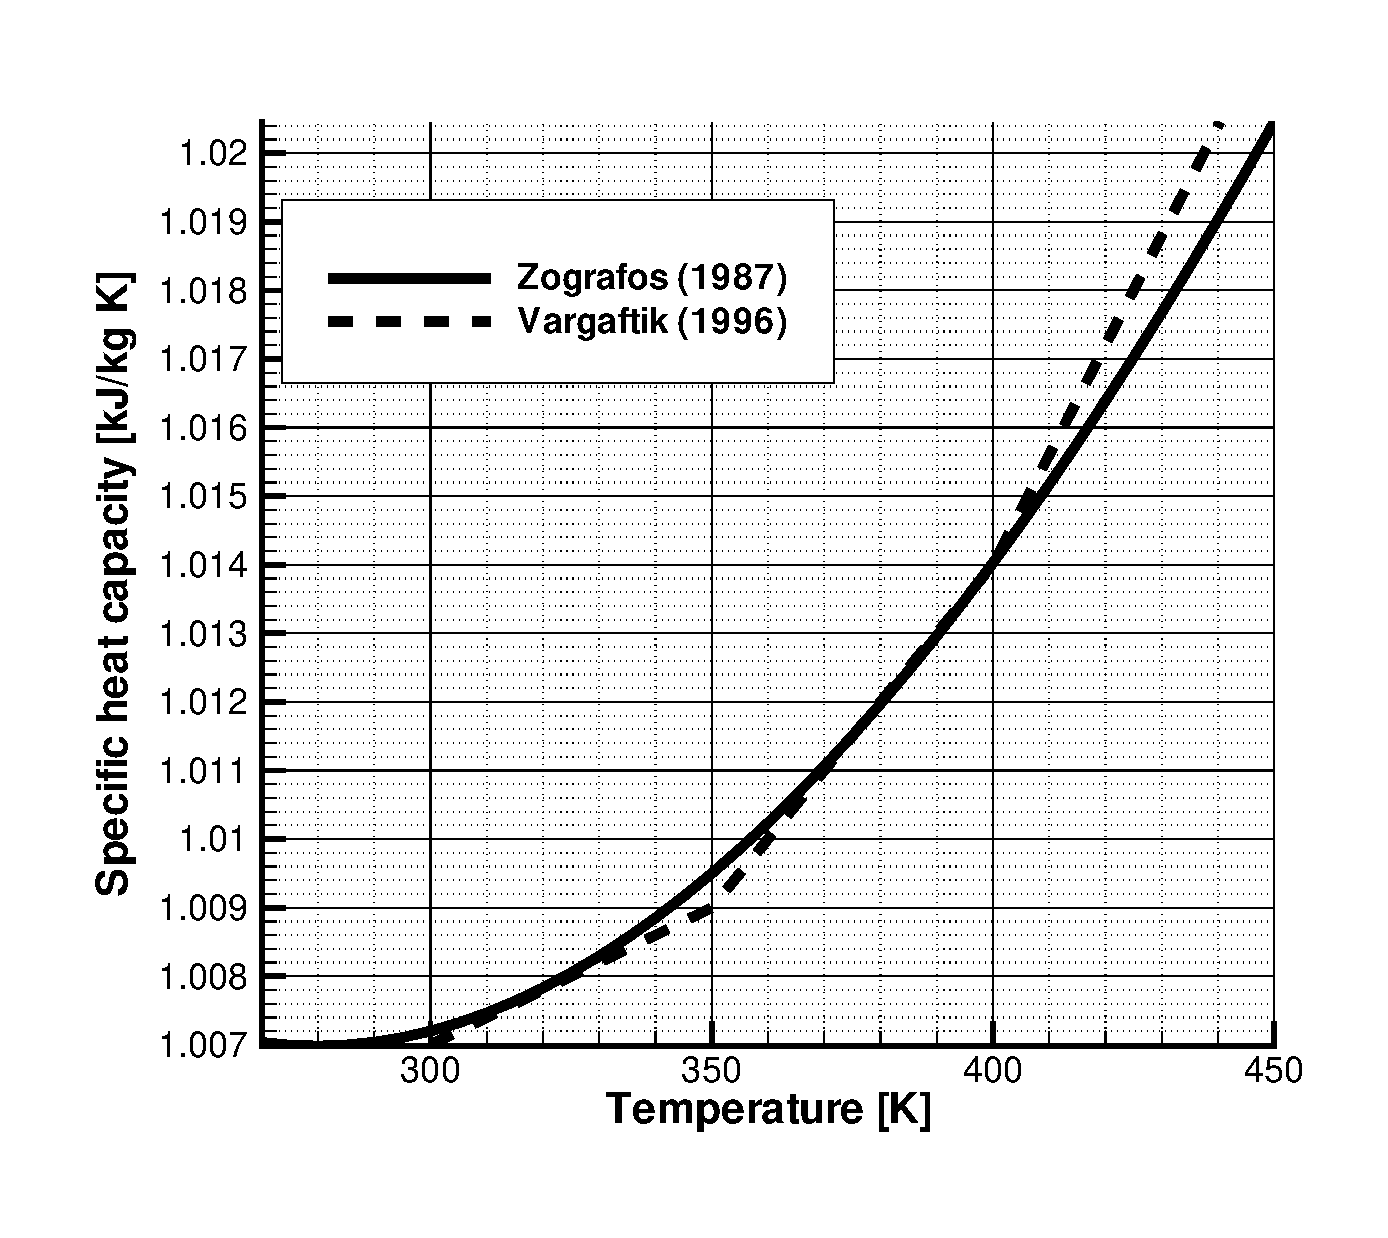
\includegraphics[width=0.49\columnwidth]{chapter20/figures/heat_capacity_air.eps}
%\centerline{Heat capacity}
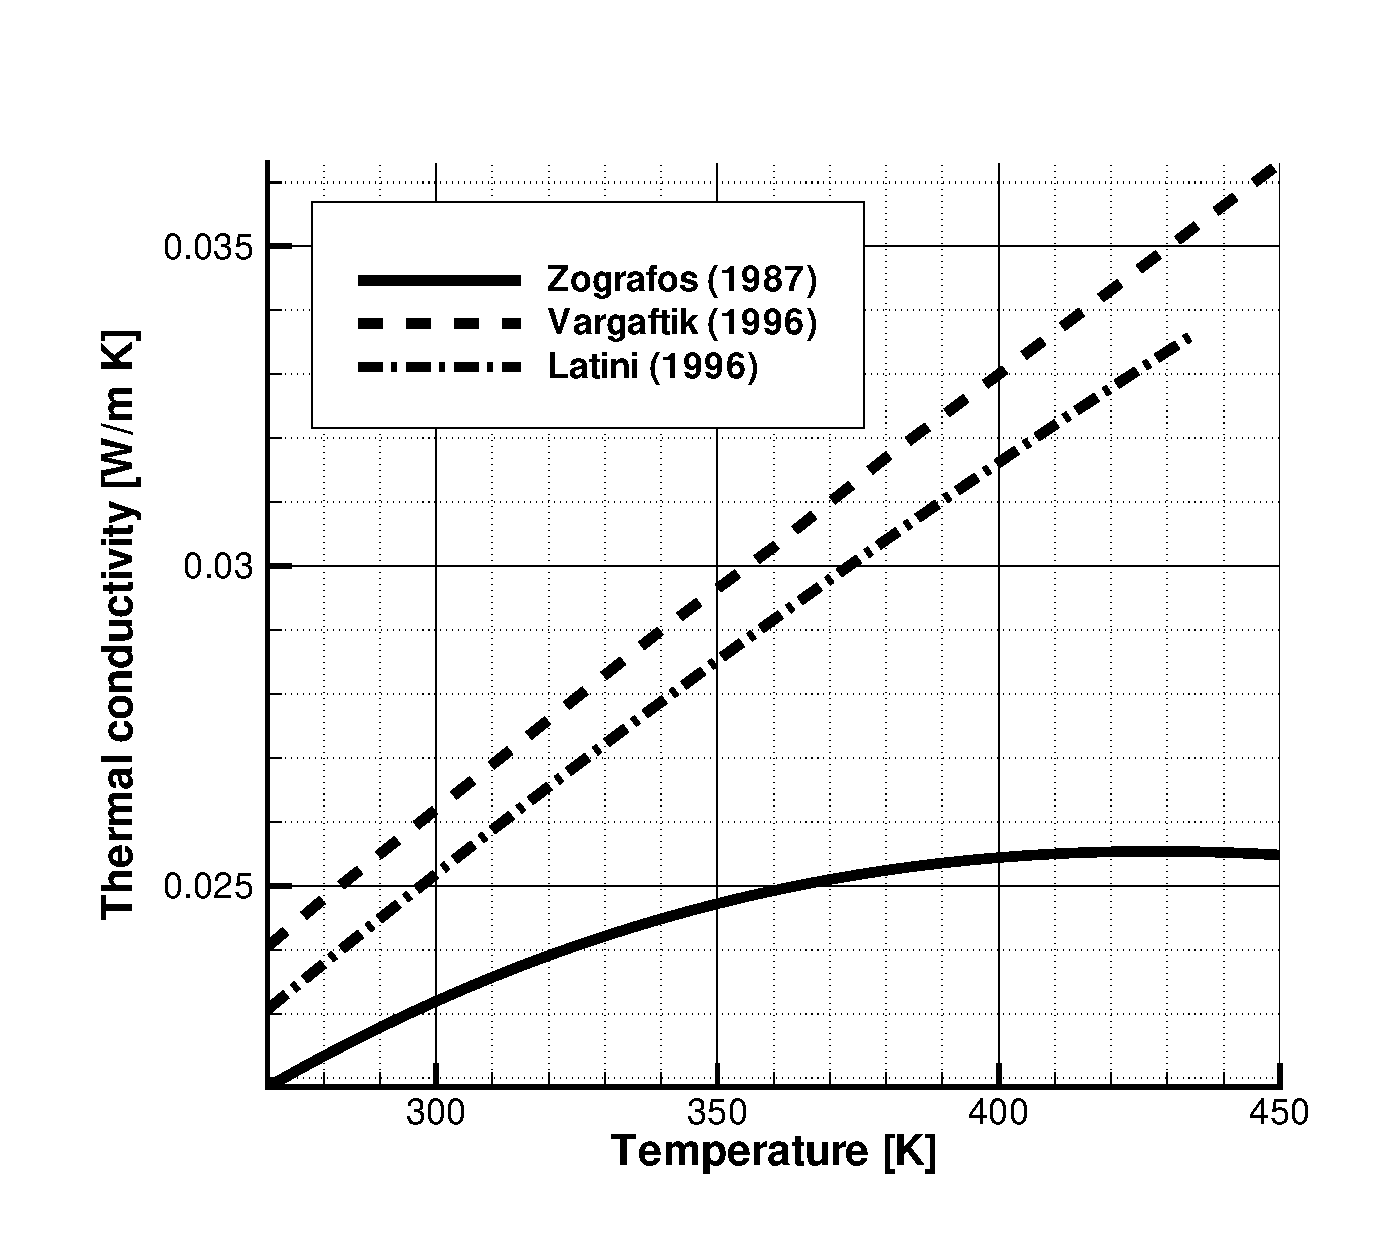
\includegraphics[width=0.49\columnwidth]{chapter20/figures/heat_conductivity_air.eps}
%\centerline{Thermal conductivity}
\end{center}
\caption{Thermal properties of air}
\label{fig:thermal_properties}
\end{figure}